\chapter{Introduction}
\label{chp:intro}

\section{Motivation}
\label{chp:intro:sec:motivation}

Mobile Security is a part of IT-Security with the focus on Mobile Devices like smartphones or tablets. The importance of mobile security highly increased since the first touchscreen devices arrived the non-business market because more and more people are using these devices to manage their data and work. \\
The users are getting used to organize the whole life on their smartphones. Data on the smartphone goes from private messages like SMS/MMS or E-Mails, over photos to nearly all accounts. Including social media accounts and the high sensitive (online) banking accounts. With the introduction of Google and Apple Pay, an hacker has one more option to damage the owner of the banking account. Also the handled Data is highly sensitive since it contains paying information.\\
But mobile devices also handling business data like your time planing or confident information in your E-Mails. A lot users have their private and business data on the same device.\\
The mobility and connectivity of modern mobile devices are a high risk. So all data should be secured in different ways.

\newpage

\section{Definition}
\label{chp:intro:sec:definition}

IT-Security is a generic term for a lot of different topics. Mobile security is a particular part of security with the same concerns but with focus on mobile devices.

\begin{figure}[h]
	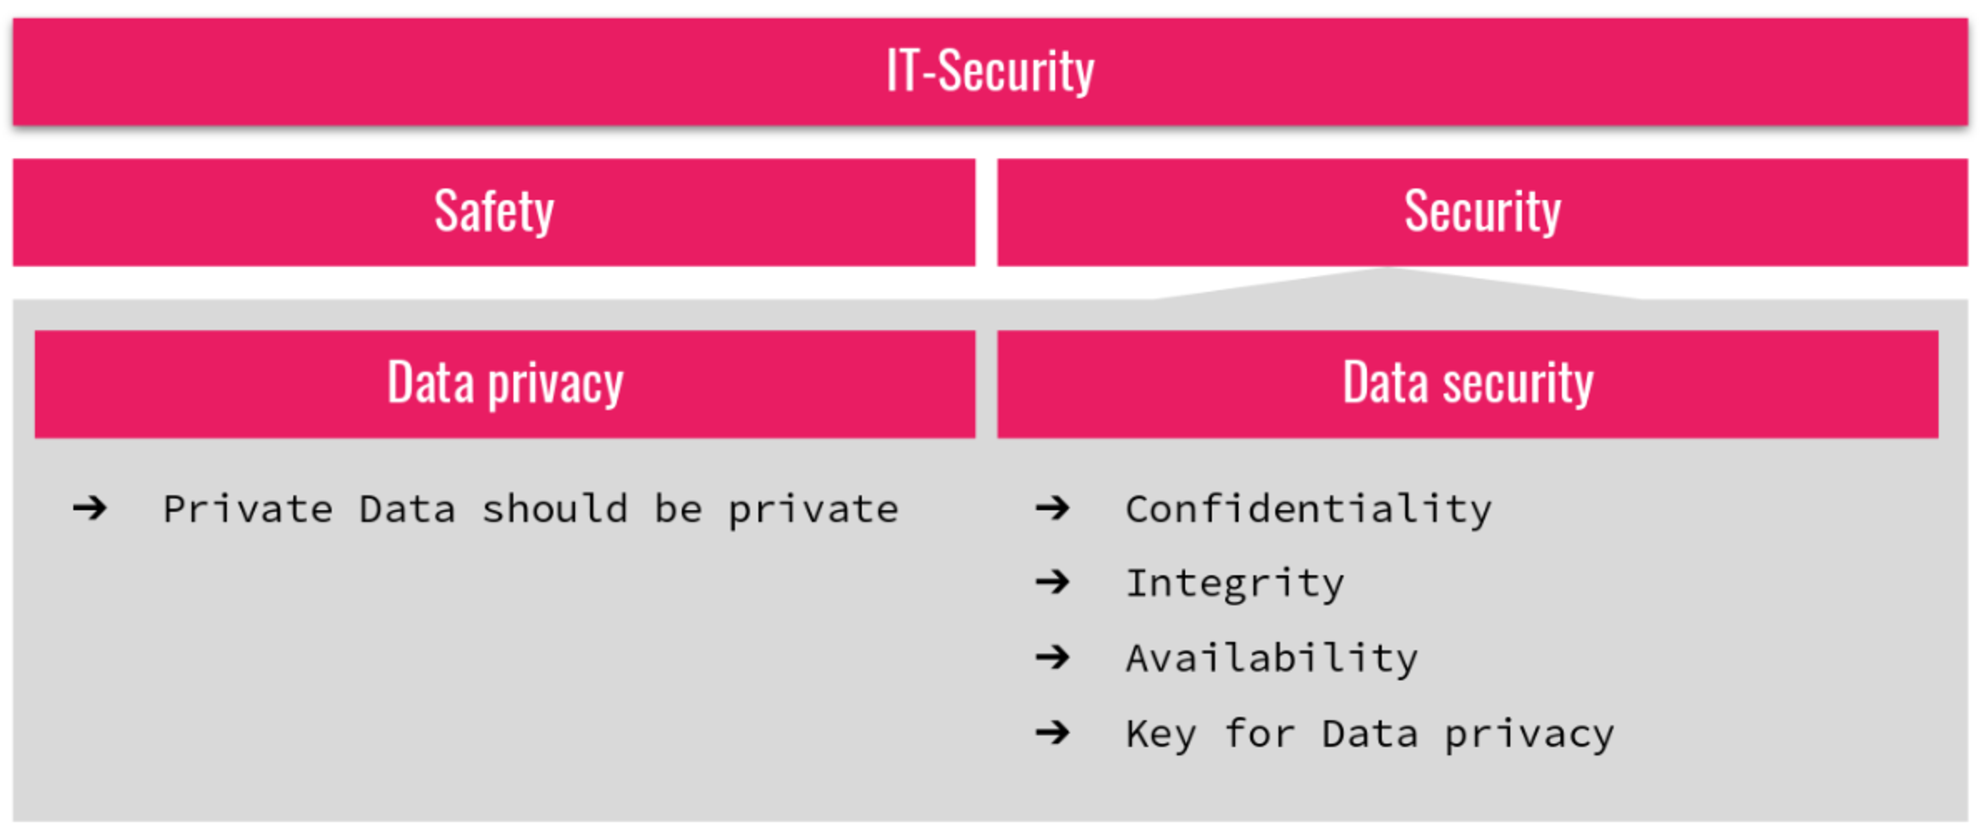
\includegraphics[width=\textwidth, angle=0]{img/it_security.pdf}
		\caption{Parts of IT-Security}
	\label{img:part_it_security}
\end{figure}

\subsection{Safety}
\label{chp:intro:sec:definition:ssec:safety}

The main question in safety is: \textit{Does my application what it is supposed to do?}. \\
So it is about functionality and often directly defined by customers or stakeholder. One strategy to avoid problems with safety topics are automated test. For example unit tests and integration test running by a continuous integration (CI). \\
But safety is not the focused topic.

\subsection{Security}
\label{chp:intro:sec:definition:ssec:safety}

Security is about information and data. Like in Fig. \ref{img:part_it_security} it can be split into privacy and security.

\subsubsection{Privacy}
\label{chp:intro:sec:definition:ssec:safety::sss:privacy}

Privacy' subject is to make sure that personal data like age, name or address are accessible only by people who are allowed. \\
Since \hyperref[https://gdpr-info.eu/]{GDPR} came into force, it is not only a ideological question it is also a lawful question. And not fulfill this law can result in very high fines.\\ The goals, to keep private data private, can only get achieved with security. 

\subsubsection{Security}
\label{chp:intro:sec:definition:ssec:safety::sss:security}

Security has three general targets.

\begin{description}
	\item[Confidentiality] is about making sure to restricted the access to a level where only people with the necessary privileges are allowed to see, change or delete these data.
	
	\item[Integrity] makes sure that every unauthorized change can be detected and changes are verifiable.
	
	\item[Availability] Means that the information should be always available to the user.
\end{description} 

But there are also some more specific target. These does not fit in every use case.

\begin{description}
	\item[Authenticity] aims on reliability. It should be clear that a message comes from the specific sender.
	
	\item[Anonymity] In some cases it should not be possible to connect a network package to a specific person.
\end{description} 

In a lot of cases it is a trade of between these targets. In this case it should be clear why and what it means to not fulfill the target to 100\%.

